\section{\METHOD~Structured Language Commands}
%\section{Structured Language Commands}
\label{section:ssl}


\begin{figure*}[t]
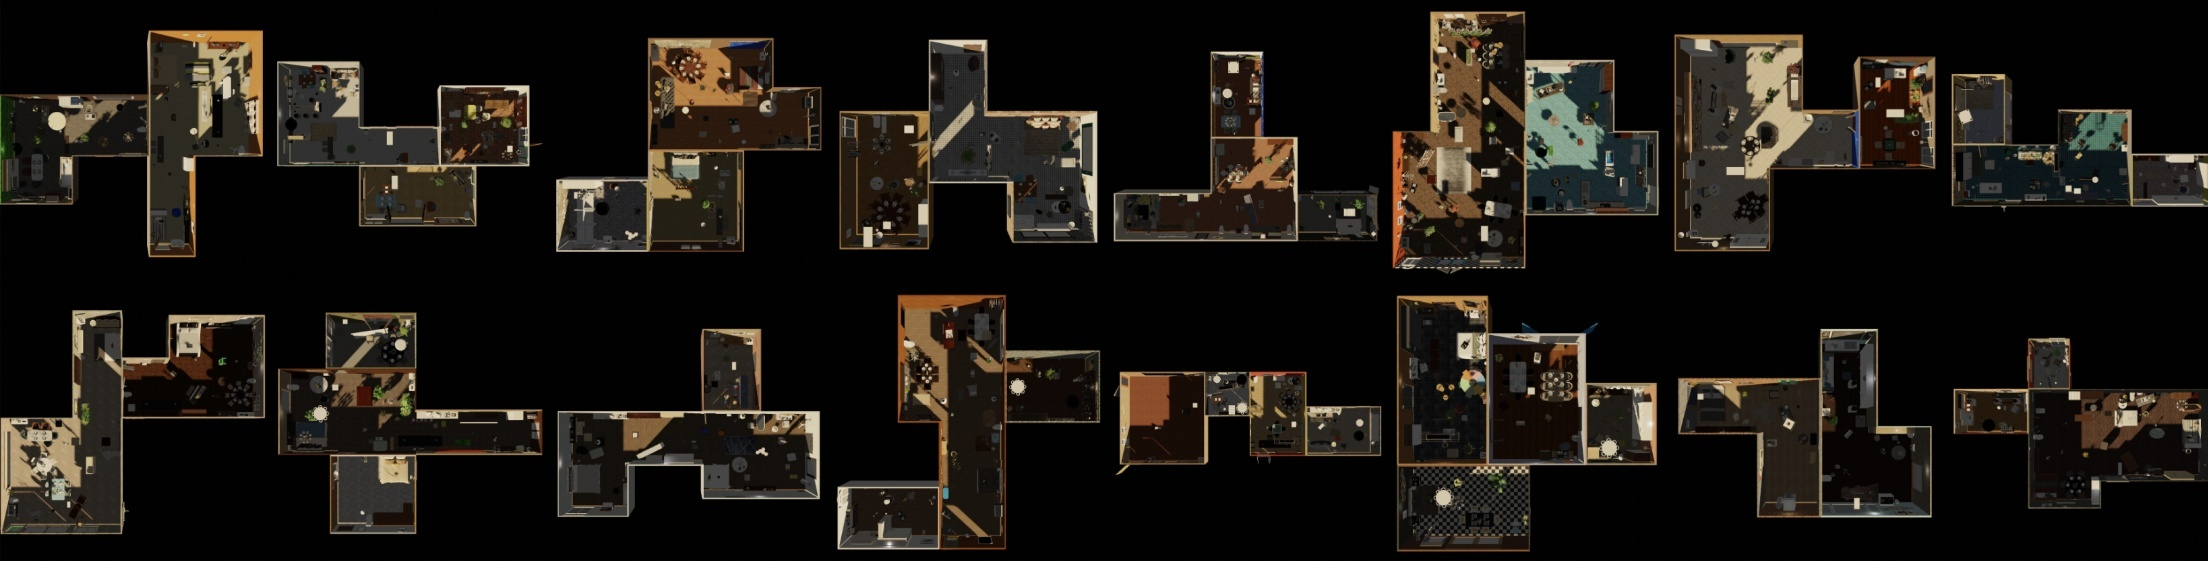
\includegraphics[width=\textwidth]{figs/ASE-2-row.jpg}
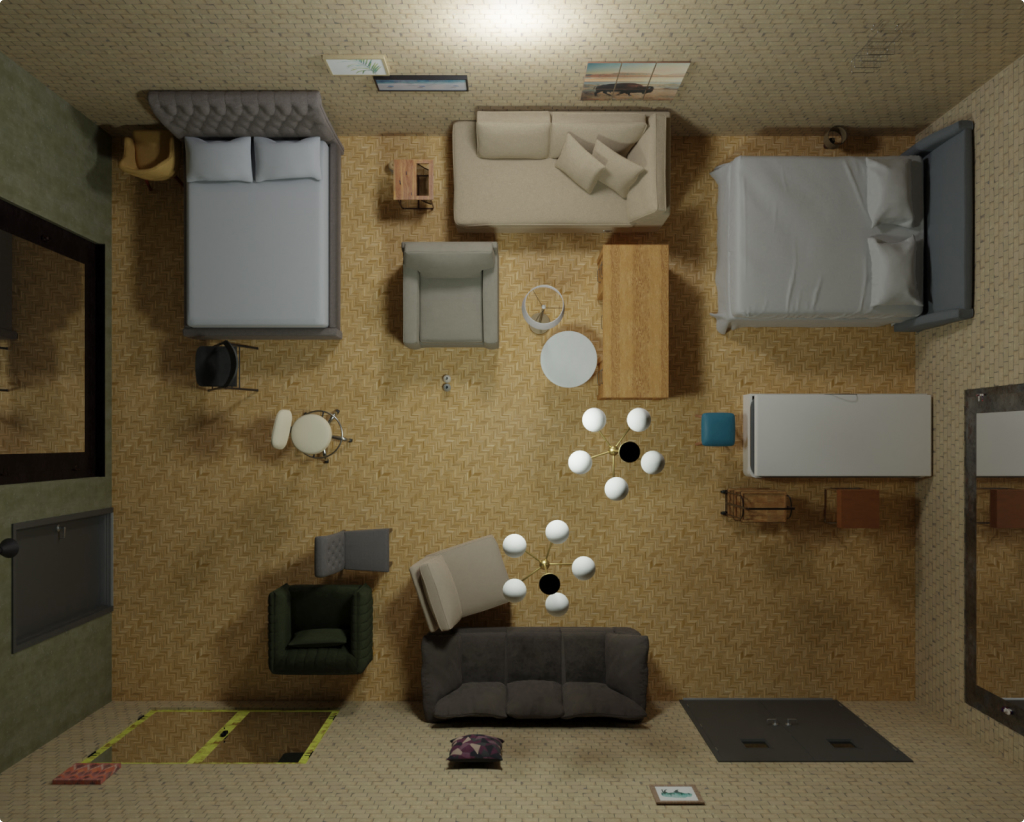
\includegraphics[width=0.245\textwidth]{figs/ase_scene_top_down.jpg} 
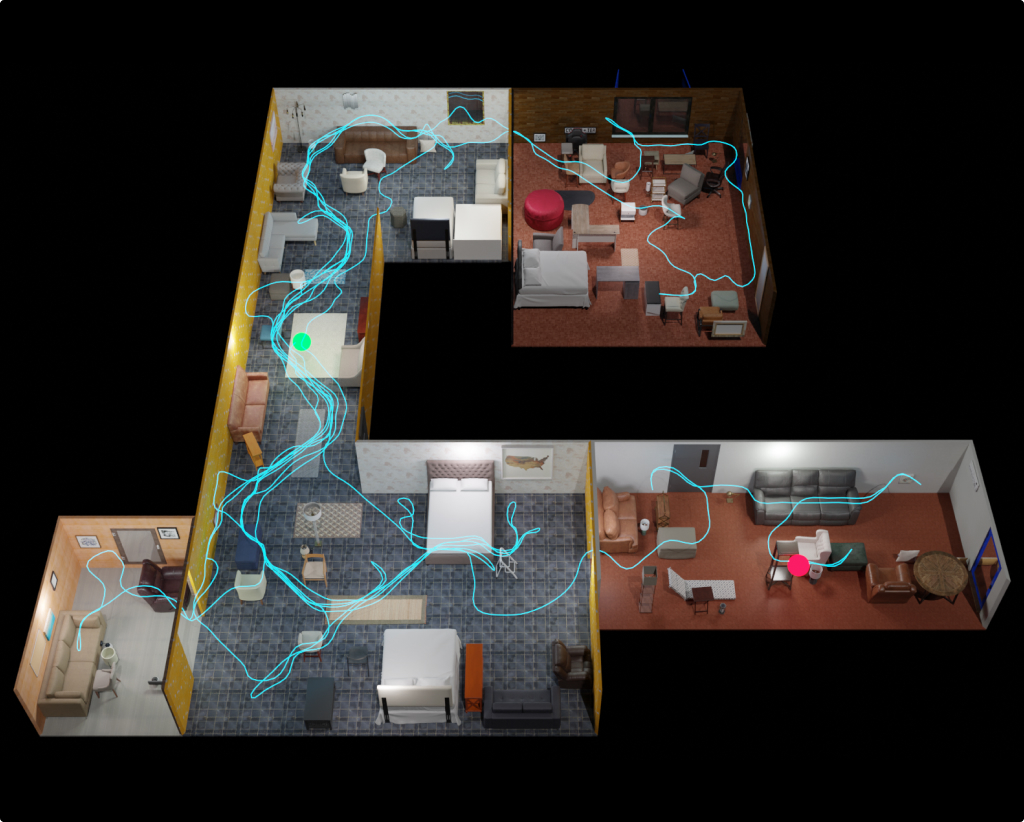
\includegraphics[width=0.245\textwidth]{figs/ase_scene_trajectory.jpg} 
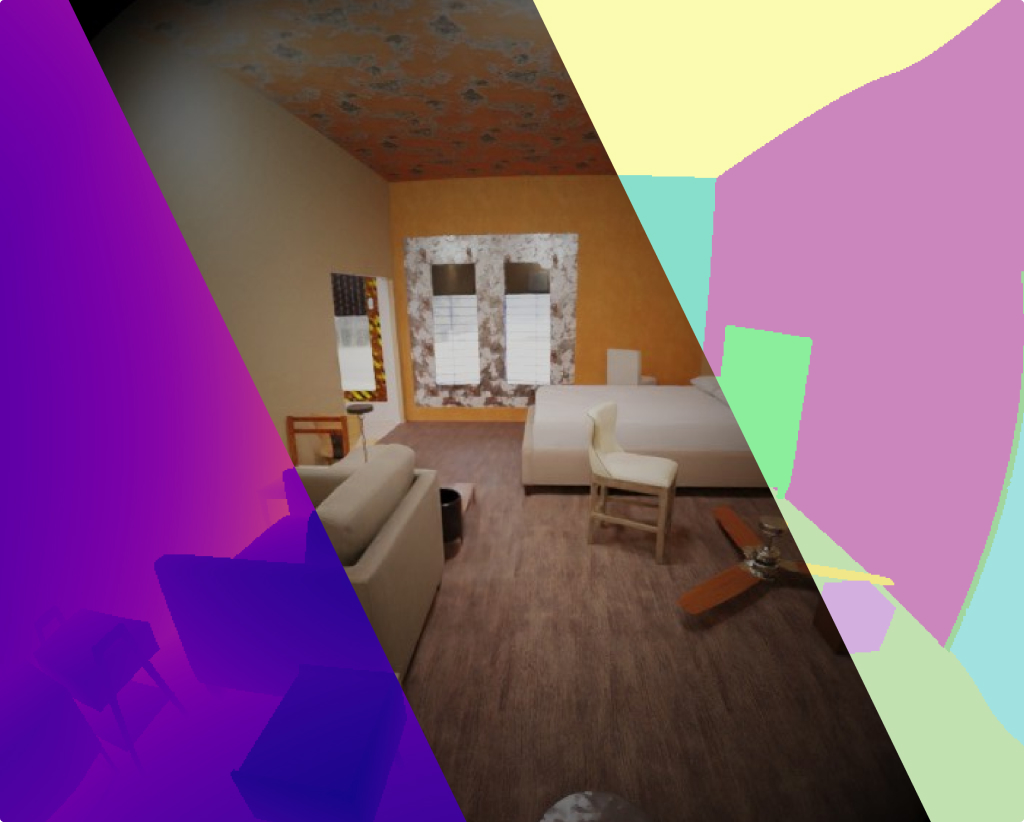
\includegraphics[width=0.245\textwidth]{figs/ase_modalities.jpg} 
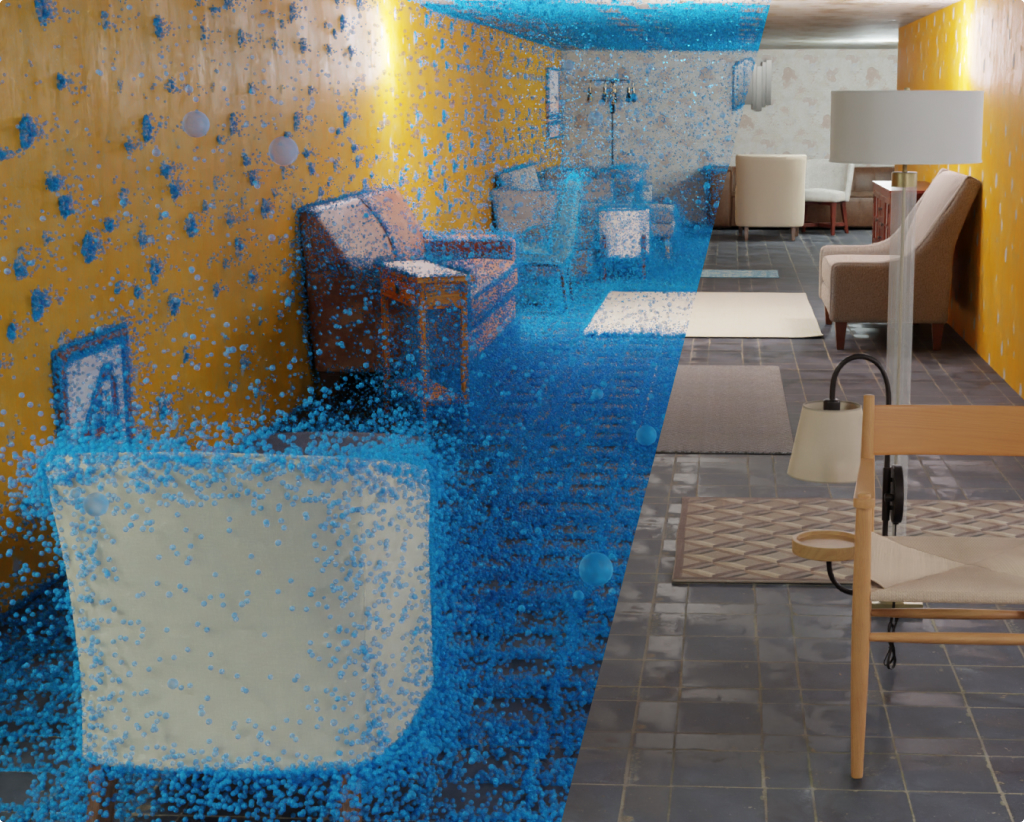
\includegraphics[width=0.245\textwidth]{figs/ase_pointcloud.jpg}
\caption{\DatasetName:
(top) Random samples of generated scenes showing diversity of layouts, lights and object placements. (bottom - left to right) A top down view of a scene filled with objects, a simulated trajectory (blue path), renderings of depth, RGB, and object instances, and lastly a scene pointcloud.}
\label{fig:dataset_teaser}
\end{figure*}



We first describe our structured language commands
that define a full scene representation including both layout and objects.
After this, we introduce our corresponding
large scale training dataset: \DatasetName{}.

\subsection{Commands and Parameters}
\label{subsec:ssl_commands}

We begin with a parameterization that captures the most common layout elements.
For this purpose we use three commands:
\texttt{make\_wall}, \texttt{make\_door}, and \texttt{make\_window}.
Each command comes with a set of parameters that results in well-defined geometry.
For example,
the full set of parameters for \texttt{make\_wall} specifies a gravity-aligned 2D plane,
while \texttt{make\_door} and \texttt{make\_window} specify box-based cutouts from walls.
It is worth noting that this parametrization is arbitrary,
and is only made in the context of presenting a proof-of-concept \METHOD~system.
There are infinitely many parametrization schemes,
in this work we opt for one that prioritizes ease of use and research iteration speed.

In addition to representing these three major layout entities, we aim to jointly infer objects as oriented bounding boxes. Thus, we introduce a fourth command:
\begin{lstlisting}[language=StructuredLanguage]
make_bbox: id, class, position_x, position_y, position_z, angle_z, scale_x, scale_y, scale_z
\end{lstlisting}
This simple parametrization represents an oriented 3D bounding box that is assumed to be aligned with gravity (assuming it points in the $-z$ direction). 
A summary of these commands and their respective parameters are shown in Table~\ref{table:commands_and_parameters}.

While we have described just four commands to capture structure and objects in an indoor environment, importantly,
this text-based parametrization can readily be extended 
geometrically and/or even semantically
to include states or other functional aspects.
% To illustrate, the parameter \texttt{wall\_idx} is a reference to a wall within the sequence and has no physical meaning.
For example,
changing the mentioned \texttt{make\_door} command
to include parameters 
% such as \lstinline[style=cmdstyle]!open_degree!
such as \texttt{open\_degree}
allows the language to represent door states.
In Section~\ref{section:extendability},
we demonstrate how such extensions to the language allows for \METHOD~to readily adapt to new tasks including coarse 3D object reconstruction.

% Someone please check that this makes sense
\subsection{Scene Definition}

A single scene can be described as a sequence of our proposed structured language commands. The sequence requires no specific ordering, and can be of arbitrary length.
From this definition, the 3D scene can easily be obtained by parsing the commands through a simple custom interpreter.



